\documentclass[../../document.tex]{subfiles}

\begin{document}
    \section{Definite Clause Programs (\abrv{dcp})}
    \abrv{Dcp} are, in contrast to \abrv{lcfrs}, a formalism where each rule produces trees instead of plain strings.
    The most striking difference to the previous formalism, however, lies in the composition expressions contained in each rule:
    They do not only allow substitution with parameters produced by successors in a derivation (first order substitution), but each single parameter may also contain variables that are substituted in the same step (second order substitution).
    This corresponds to the information flow from bottom to the top in a derivation as expressed by synthetic attributes (first order substitution), as well as the information flow from top to the bottom in a derivation by inherent attributes (second order substitution) in attribute grammars.
    The implementation of these two systems of substitution, two pairwise distinct sets of variables are used: \(\X\) for the first (as in \abrv{lcfrs}), and \(\Y\) for the second order substitution.

    In their most general form, the object produced by a derivation in such a \abrv{dcp} is not necessarily computable, as the two types of substitution may mutually recur.
    To solve this issue, there were some restrictive forms introduced which exclude circular dependencies in the expressed productions. \citep[Sec.~3.4 about non-circular attribute grammars]{Cou82}
    It is easy to see that the definition shown in this section supersedes each of these restricted forms, as it exclusively allows fixed terminal objects or a single second order variable as parameter for second order substitution.
    To avoid unnecessarily complicated definitions, the subset of \abrv{dcp} shown in this section is even further restricted such that
    \begin{inparaenum}
        \item each composition yields one sequence of consecutive trees (and not sequences of ranges) that is a subforest in the parse, and
        \item each rule's composition expression allows exactly one second-order substitution (which may be the empty sequence).
    \end{inparaenum}

    \begin{definition}[Composition]
        We fix the \(\DN\)-family of finite sets of variables \((\X_k = \{\x_i \mid i \in [k]\} \mid k \in \DN)\), and the singleton set \(\Y = \{\y\}\).
        The identifier \(\X\) denotes the union \(\bigcup_{k \in \DN} \X_k = \{\x_i \mid i \in \DN\}\).
        Let \(\varSigma\) and \(\varGamma\) be alphabets disjoint from \(\X \cup \Y\).
        The \(\DN\)-family \((S_k = \{x(y) \mid x \in \X_k, y \in \T_\varGamma(\varSigma \cup Y)^*\} \mid k \in \DN)\) denotes expressions for occurrences of first-order substitutions using \(k\) variables.
        The \(\DN\)-family of \abrv{dcp} \deflab<\dcp>[dcp:comp]{composition}[compositions] over \(\varSigma\) and \(\varGamma\) is \((\C^{\varGamma\varSigma}_k \mid k \in \DN)\) such that \(\C^{\varGamma\varSigma}_k\) contains each nonempty sequence \(c\) in \((\T_\varGamma(\varSigma \cup \Y \cup S_k))^+\) such that each variable in \(\X_k \cup \Y\) occurs exactly once in \(c\).
        We associate the identifier \(\C^{\varGamma\varSigma}\) with the set of all such \abrv{dcp} compositions \(\bigcup_{k \in \DN} \C^{\varGamma\varSigma}_{k}\).

        Each composition \(c \in \C^{\varGamma\varSigma}_k\) is associated with a function \[
        \sem{c}\colon \big(\T_\varGamma(\varSigma \cup Y)^*\big)^k \to \T_\varGamma(\varSigma \cup Y)^*
        \] such that \(\sem{c}(\xi_1, \ldots, \xi_k) = c[\x_1=\xi_1, \ldots, \x_k=\xi_k]\) is the second-order substitution of \(\X_k\) in \(c\).
    \end{definition}

    %    The occurrences of variables are abbreviated in the following two ways:
    %    \begin{compactenum}
        %        \item Variables in \(\X\) with successor \(\varepsilon\) are abbreviated by omitting the parentheses and the successor as a whole; e.g.\@ instead of \(\x_1(\varepsilon)\), we just write \(\x_1\).
        %        \item We omit trailing occurrences of the variable \(\y\), if it does not occur as a successor of any node; e.g.\@ instead of \(\text{S}(\x_1)\,\y \), we just write \(\text{S}(\x_1)\).
        %    \end{compactenum}

    \begin{example}\label{ex:dcp:comp}
        Consider the following compositions over the alphabets \(\varSigma = \{ \cn{sbar}, \cn{s}, \cn{vp}, \cn{np} \}\) and \(\varGamma = \{\tn{where}, \tn{the}, \tn{survey}, \tn{was}, \tn{carried}, \tn{out}\}\):
        \begin{align*}
            c_1 &= \tn{where} \, \y,
            &c_2 &= \y \, \tn{out},
            &c_3 &= \cn{np} (\y \, \tn{survey}) && \in \C_0\\
            c_4 &= \cn{vp}(\x_1(\y) \, \tn{was}) && && && \in \C_1 \\
            c_5 &= \cn{sbar} (\cn{s} (\x_1(\y) \, \x_2(\tn{the}))),
            &c_6 &= \cn{vp}(\x_1(\y) \, \x_2(\tn{carried})) && && \in \C_2
        \end{align*}
        The subscript indexing the family of compositions \(\C\) determines the number of arguments for the functions represented by the elements in \(\C\).
        E.g.\@ \(\sem{c_1}\) takes no arguments, and \(\sem{c_6}\) takes two arguments.
        Evaluating any term of such compositions yields a sequence tree in \(\T_\varSigma(\varGamma \cup \Y)\) with exactly one occurrence of \(\y\), for example:
        \begin{align*}
            \sem{c_6} \big( \sem{c_1}(), \sem{c_2}() \big)
            &= \sem{c_6} \big( \: (\tn{where} \, \y), \: (\y \, \tn{out}) \: \big) \\
            &= \cn{vp}(\x_1(\y) \, \x_2(\tn{carried}))[\x_1=(\tn{where} \, \y), \x_2=(\y \, \tn{out})] \\
            &= \cn{vp}(\x_1 \, \x_2)[\x_1=(\tn{where} \, \y)[\y=\y], \x_2=(\y \, \tn{out})[\y=\tn{carried}]] \\
            &= \cn{vp}(\x_1 \, \x_2)[\x_1=(\tn{where} \, \y), \x_2=(\tn{carried out})] \\
            &= \cn{vp}(\tn{where} \, \y \, \tn{carried out})
        \end{align*}
    \end{example}

    \begin{definition}[\abrv{Dcp} Grammar]
        A \deflab[dcp]{definite clause program}%
        \defabrv{\dcp}{\abrv{dcp}}
        is a tuple \(G=(N, \varGamma, \varSigma, S, R)\) where
        \begin{compactenum}
            \item \(N\) is a finite set (\emph{nonterminals}),
            \item \(\varGamma\) and \(\varSigma\) are alphabets (\emph{terminals}),
            \item \(S \in N\) (\emph{initial non-terminal}),
            \item \(R\) is a finite subset of \(\bigcup_{k \in \DN} N \times \C^{\varGamma\varSigma}_k \times N^k\) (\deflab<\dcp>{rule}[rules]). % such that for each rule \((A, c, B_1\cdots B_k)\) holds: if \(A = S\) then \(c\) is of length 1.
        \end{compactenum}

        Rules are denoted in the form \(A \to c\,(B_1, \ldots, B_k)\) instead of \((A, c, B_1 \cdots B_k)\); \(A\) is called the \abrv{lhs} and \(B_1, \ldots B_k\) are the \abrv{rhs}, \(c\) is the composition of the rule.
        The natural \(k\) is the \deflab<\dcp!rule>{rank} of the rule; the rank of the grammar \(G\) is the maximum rank occurring in the rules of \(G\).
    \end{definition}

    \begin{definition}[\abrv{Dcp} Grammar Forms]
        The concepts around rule and grammar forms are equal in \abrv{lcfrs} and \abrv{dcp}:
        \begin{compactitem}
            \item Rules are called \deflab<\dcp!rule>{nullary}, \deflab<\dcp!rule>{unary} and \deflab<\dcp!rule>{binary} according to their rank.
            \item A grammar that contains only rules of rank \(\leq 2\) is called \deflab<\dcp>{binary}.
            \item A rule whose composition contains exactly one symbol in \(\varGamma\) is called \deflab<\dcp!rule>{lexixal}.
            \item A grammar that contains only lexical rules is called \deflab<\dcp>{lexical}.
            \item A rule that does not contain any symbol in \(\varGamma\) is called \deflab<\dcp!rule>{non-lexical}.
        \end{compactitem}
    \end{definition}

    The concept of derivations in \abrv{dcp} is equal to those in \abrv{lcfrs}.
    However, the terms yield and parse differ, since the grammar produces trees instead of strings.
    We cannot easily enforce that compositions for a start nonterminal produce a single tree.
    Therefore, the definition introduces a fresh symbol \(\cn{root}\) that governs the sequence of trees produced by the compositions of a derivation.

    \begin{definition}[Derivation, Yield and Parse]
        A \deflab<\dcp>{derivation} in a \abrv{dcp} \(G = (N, \varSigma, S, R)\) is a tree in \(\T_R\) such that each node's \abrv{rhs} nonterminals match the \abrv{lhs} nonterminals of its children.
        The family of derivations \((\derivs^R_A \mid A \in N)\) is defined such that \(\derivs^R_A\) contains all derivations where the root is equipped with the \abrv{lhs} nonterminal \(A\).
        The set of all derivations is \(\derivs^R = \bigcup_{A \in N} \derivs^R_A\).

        Consider a derivation \(d\) in \(\derivs^R_A\) of the form \(d = r\,(d_1, \ldots, d_k)\) where the root \(r\) is of the form \(A \to c\,(B_1, \ldots, B_k)\).
        We fix a symbol \(\cn{root}\) that is not in \(\varGamma \cup \varSigma\) and define the \deflab<\dcp!derivation>[dcp:parse]{parse} of \(d\) as the tree \[
        \parse(d) = \cn{root}\Big( \sem{c}(\parse(d_1),\ldots,\parse(d_k))[\y=\varepsilon]\Big) \text{.}
        \]
        The \deflab<\dcp!derivation>[dcp:yd]{yield} of \(d\) is \(\yield(d) = \yield(\parse(d))\).
    \end{definition}

    \begin{example}[Continues \cref{ex:dcp:comp}]
        Consider the alphabet \(N = \{\nt{v}^\nt{L}, \nt{v}, \nt{n}, \nt{s} \}\) and the \abrv{dcp} \(G = (N, \varSigma, \nt{s}, R)\) where
        \begin{align*}
            R = \Big\{ \quad
            \nt{v}^\nt{L} &\to (\tn{where} \, \y)\:(),
            \quad \nt{v} \to (\y \, \tn{out})\:(),
            &\nt{n} &\to (\cn{np} (\y \, \tn{survey}))\:(), \\
            \nt{v} &\to (\cn{vp}(\x_1(\y) \, \tn{was}))\:(\nt{v}),  \\
            \nt{s} &\to (\cn{sbar} (\cn{s} (\x_1(\y) \, \x_2(\tn{the}))))\:(\nt{v}, \nt{n}),
            &\nt{v} &\to (\cn{vp}(\x_1(\y) \, \x_2(\tn{carried})))\:(\nt{v}^\nt{L}, \nt{v})
            \quad \Big\} \text{.}
        \end{align*}

        The tree \(d\) illustrated below (left) is a derivation in \(\derivs^R_\nt{v}\), its parse is shown to the right of \(d\).
        A part of the computations (for the bottom \(\cn{vp}\)-node) was already shown in the previous example in detail.
        We can read the yield of \(d\) from the leave of the parse: \(\tn{where carried out was}\).

        \null\hfill
        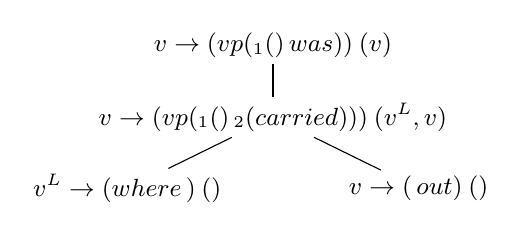
\begin{tikzpicture}[level distance=6ex, font=\small, sibling distance=3.7cm, inner sep=2pt]
            \node {\(\nt{v} \to (\cn{vp}(\x_1(\y) \, \tn{was}))\:(\nt{v})\)}
            child {node {\(\nt{v} \to (\cn{vp}(\x_1(\y) \, \x_2(\tn{carried})))\:(\nt{v}^\nt{L}, \nt{v})\)}
                child {node {\(\nt{v}^\nt{L} \to (\tn{where} \, \y)\:()\)}}
                child {node {\(\nt{v} \to (\y \, \tn{out})\:()\)}}};
        \end{tikzpicture}
        \hfill
        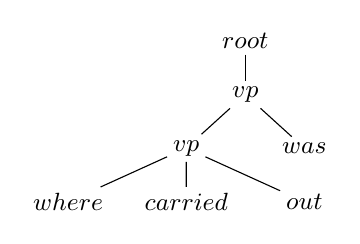
\begin{tikzpicture}[level distance=4.5ex, font=\small, inner sep=2pt]
            \node {\(\cn{root}\)}
            child{ node {\(\cn{vp}\)}
                child {node {\(\cn{vp}\)}
                    child {node {\(\tn{where}\)}}
                    child {node {\(\tn{carried}\)}}
                    child {node {\(\tn{out}\)}}}
                child {node {\(\tn{was}\)}}};
        \end{tikzpicture}
        \hfill\null
    \end{example}
\end{document}